\newpage
\section{Amplificador VFA - VFA:}
\hspace{1mm} Las especificaciones del VFA LM324 se detallan a continuación.

\begin{itemize}[itemsep=1pt]
    \item $A_{d0}=100~dB$
    \item $f_T=1~MHz$
    \item $f_1=10~Hz$
    \item $f_2=5.06~MHz$
\end{itemize}

 
\hspace{1mm} Considerando AO2 como ideal, se calcularan las ganancias de lazo abierto $Ad(s)$, ganancia de lazo $T(s)$ y ganancia de lazo cerrado $Avf(s)$. Posteriormente, se procederá a compensar el sistema para lograr una máxima planicidad de módulo como se solicita.

\begin{figure}[H]
    \centering
    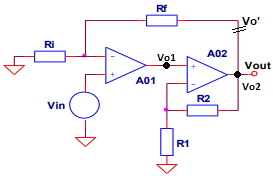
\includegraphics[scale=1.2]{figuras/6. Punto1LazoCerradoVoP.png}
    \caption{Amplificador compuesto VFA-VFA}
\end{figure}

\subsection{Análisis teórico}
\subsubsection {Ganancia de Lazo Abierto}

\hspace{1mm} Es la relación entre la tensión de salida y la tensión de entrada.

\begin{equation}
    Av(s) = \frac{V_{out}}{V_{in}} 
\end{equation}

\hspace{1mm} Por un lado, se tiene

\begin{equation}
    V_{o1} = Ad(s)\cdot V_{in} 
\end{equation}

\hspace{1mm} Además

\begin{align}
    V_{o} &= \left(1+\frac{R_2}{R_1}\right) \cdot V_{o1} \\
          &= \left(1+\frac{R_2}{R_1}\right) \cdot Ad(s) \cdot V_{in}
\end{align}

\hspace{1mm} Por lo tanto

\begin{equation}
 \boxed{Av(s) = \left(1+\frac{R_2}{R_1}\right) \cdot Ad(s)}
\end{equation}

 
\hspace{1mm} Con la ayuda de la herramienta Matlab, se graficó el diagrama de Bode de la función de transferencia a lazo abierto del amplificador compuesto real. En él, es posible observar los polos en $10~Hz$ y en $5.06~MHz$.


\begin{figure}[H]
    \centering
    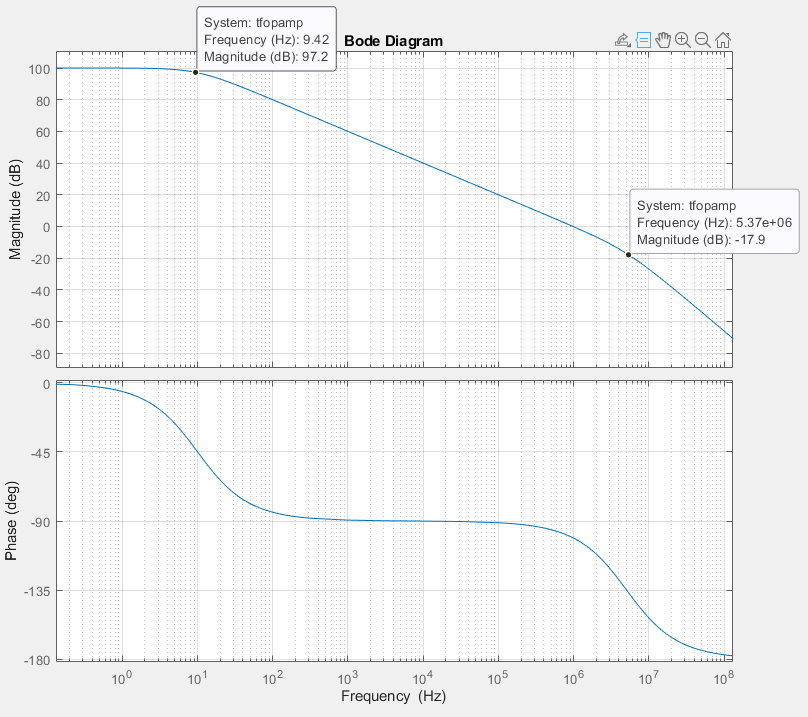
\includegraphics[width=0.9\linewidth]{figuras/7. Opamp_real_lazoabierto.png}
    \caption{Diagrama de Bode del amplificador lazo abierto}
\end{figure}


\subsubsection {Ganancia de Lazo T}
\begin{align}
    T(s) &= \frac{V_{out}}{V_{out'}}|_{V_{in}=0} \\
    T(s) &= \frac{V_{out}}{V_{o1}} \cdot \frac{V_{o1}}{V_{1}-} \cdot \frac{V_{1}-}{V_{out'}}\\
    T(s) &= \left(1+\frac{R_2}{R_1}\right) \cdot (-Ad(s)) \cdot \left(\frac{R_i}{R_i+R_f}\right)
\end{align}

\hspace{1mm} Entonces,
\begin{equation}
 \boxed
 {T(s) = -Ad(s) \cdot \left(1+\frac{R_2}{R_1}\right) \cdot \left(\frac{R_i}{R_i+R_f}\right)}
\end{equation}

\subsubsection {Ganancia de Lazo Cerrado}
\begin{equation}
    Avf(s) = \frac{Av(s)}{1-T}
\end{equation}

\hspace{1mm} Reemplazando se llega a
\begin{align}
    Avf(s) &= \frac{\left(1+\frac{R_2}{R_1}\right) \cdot Ad(s)}{1+Ad(s) \cdot \left(1+\frac{R_2}{R_1}\right) \cdot \left(\frac{R_i}{R_i+R_f}\right)} \label{eq:primera} \\
   \nonumber
   \\
     &= \frac{\left(1+\frac{R_2}{R_1}\right)}{\frac{1}{Ad(s)} + \left(1+\frac{R_2}{R_1}\right) \cdot \left(\frac{R_i}{R_i+R_f}\right)} 
\end{align}

\hspace{1mm} Considerando la ganancia $Ad(s)$ que tiende a ser muy grande o infinita, se simplifican los cálculos

\begin{equation}
    Avf(s) = \frac{\cancel{\left(1+\frac{R_2}{R_1}\right)}}{\cancel{\left(1+\frac{R_2}{R_1}\right)} \cdot \left(\frac{R_i}{R_i+R_f}\right)} 
\end{equation}

\hspace{1mm} Por lo tanto

\begin{equation}
    \boxed{Avf(s)=\frac{R_i+R_f}{R_i}}
\end{equation}

 
\hspace{1mm} La consigna define que la ganancia de lazo cerrado debe ser $Avf(s)=20~dB$. Con dicho dato, es posible obtener la relación entre las resistencias $R_i$ y $R_f$.

\begin{equation}
    Avf(s)=20~dB \hspace{3mm} \therefore \hspace{3mm} \frac{R_i+R_f}{R_i}=20~dB = 10~veces
\end{equation}

 
\hspace{1mm} Despejando la relación de resistencias,

 
\begin{equation}
    \frac{R_f}{R_i} = 9
\end{equation}

 
\hspace{1mm} Colocando valores arbitrarios de resistencias para cumplir con la relación, se llega a:

\begin{equation}
    \boxed{
    \begin{aligned}
        &R_i=10~\text{k}\Omega \\
        &R_f=90~\text{k}\Omega
    \end{aligned}
    }
\end{equation}

 
\hspace{1mm} Además, a lazo cerrado se identifica un polo en $f_g$, el cual está estrechamente vinculado con la ganancia del amplificador AO2. Por otro lado, cumplir con la condición de máxima planicidad de módulo implica que $M\varphi =65^\circ$. En este contexto y considerando AO2 como un amplificador ideal, se procede a calcular el valor de $f_g$

\begin{equation}
    M \varphi = 180^o - arctg \left( \frac{f_g}{f_1} \right) - arctg \left( \frac{f_g}{f_2} \right) = 65,5^o
\end{equation}

\hspace{1mm} Dado que $f_g \gg f_1 \xrightarrow{} \arctan\left(\frac{f_g}{f_1}\right) \approx 90^\circ$

\begin{align}
     \Longrightarrow 180^o - 90^o - arctg \left( \frac{f_g}{f_2} \right) &= 65,5^o\\
     24.5^o &=arctg\left( \frac{f_g}{f_2} \right)\\
     tg(24.5^o) &= \frac{f_g}{f_2}= \frac{f_g}{5.06~MHz}
\end{align}

\begin{equation}
    \boxed{f_g = 2,306~MHz}
\end{equation}

\bigskip
\hspace{1mm} Con este valor calculado, se determinó la ganancia a lazo cerrado del amplificador AO2 ideal. Recordando que la consigna especificaba que $Avfi=20~dB$ y que $Ad_o=100~dB$:

\begin{align}
    Avf_{2i}&=\frac{Avfi \cdot \omega_{gi}}{Ad_0 \cdot \omega_1} =\frac{10~veces \cdot 2\pi\cdot 2,306~MHz}{100000~veces\cdot 2\pi\cdot10~Hz} \label{eq:primera} \\
   \nonumber
   \\
    Avf_{2i}&=23.06~veces =27.26~dB
\end{align}

 
\hspace{1mm} Siendo $ \omega _1 $ la frecuencia del primer polo, especificada en frecuencia angular. Finalmente, la ganancia del amplificador compuesto resulta

\begin{equation}
    Av_{comp}=Ad0\cdot Avf_{2i}=100~dB \cdot 27.25~dB
\end{equation}

\begin{equation}
    \boxed{
    Av_{comp} = 127.21~dB
    }
\end{equation}

\begin{figure}[H]
    \centering
    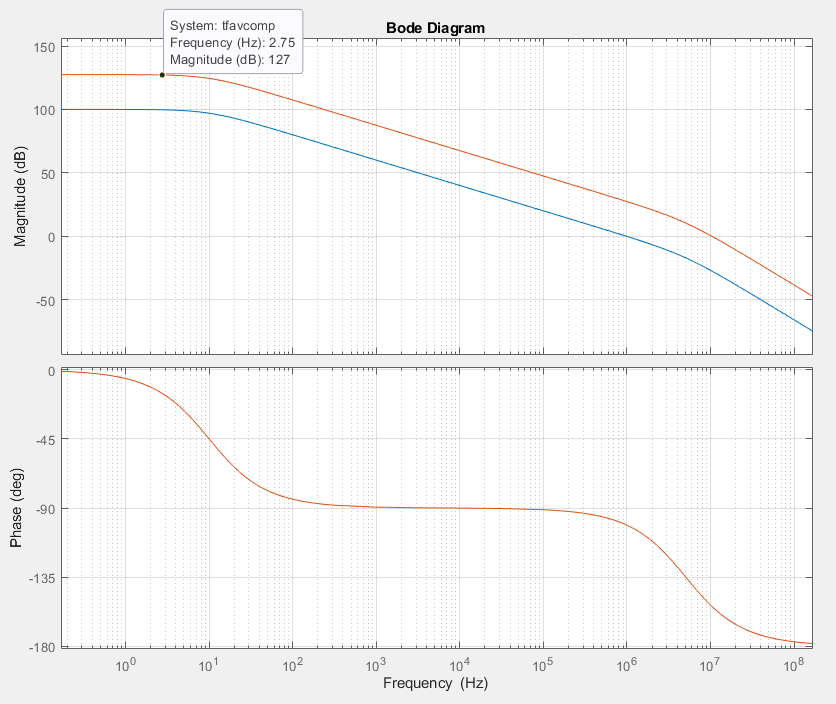
\includegraphics[width=0.9\linewidth]{figuras/8. Av_comp.png}
    \caption{Diagrama de Bode del amplificador compuesto}
\end{figure}

\hspace{1mm} En este punto, es posible obtener el valor de las resistencias $R_1$ y $R_2$

\begin{equation}
    Avf_{2i}=27.26~dB \hspace{3mm} \therefore \hspace{3mm} \frac{R_1+R_2}{R_1}=27.26~dB = 23.06~veces
\end{equation}

\hspace{1mm} Despejando la relación de resistencias,

\begin{equation}
    \frac{R_2}{R_1} = 22.06
\end{equation}

\hspace{1mm} Colocando valores arbitrarios de resistencias para cumplir con la relación, se llega a:

\begin{equation}
    \boxed{
    \begin{aligned}
        &R_1=1~\text{k}\Omega \\
        &R_2=22~\text{k}\Omega
    \end{aligned}
    }
\end{equation}


 
\hspace{1mm} Luego, se halló la función de transferencia de lazo cerrado del amplificador compuesto $(Avf_{comp})$. Para esto, se comenzó determinando la ganancia de ruido global $ K(global) $.

\begin{equation}
    K (global) = \frac{1}{Avf_{comp_i}} = \frac{1}{20~dB}
\end{equation}

\begin{equation}
    \boxed{
    K (global) = 0.1
    }
\end{equation}

 
\hspace{1mm} Se resolvió así la función de transferencia mencionada.

\begin{align}
    Ft_{Avf (comp)} &= \frac{Ad_0 \cdot Avf_{2i} \cdot \omega_1 \cdot \omega_2}{s^2 + s \cdot (\omega_1 + \omega_2) + (\omega_1 \cdot \omega_2 + K (global) \cdot Ad_0 \cdot Avf_{2i} \cdot \omega_1 \cdot \omega_2)}\\
    \\
    &= \frac{4.713 \times 10^{15}}{s^2 + 3.179 \times 10^7 s + 4,713 \times 10^14}
\end{align}

 
\hspace{1mm} Dicha función de transferencia se comparó con la ecuación base.

\begin{equation}
    \frac{\omega _p^2}{s^2 + s \frac{\omega _p}{Q_p } + \omega_p^2}
\end{equation}  

 
\hspace{1mm} Se igualaron las ecuaciones y se determinaron los siguientes parámetros.

\begin{equation}
    \omega _p ^2 = 4,713 \times 10^{14} \Longrightarrow \omega_p =\sqrt{4.713 \times 10^{14}} 
\end{equation}

\begin{equation}
    \boxed{
        \omega_p = 2.17 \times 10^7
    }
\end{equation}

\hspace{1mm} Siendo entonces la frecuencia del polo compensado:

\begin{equation}
    f_p = \frac{\omega_p}{2\pi}
\end{equation}

\begin{equation}
    \boxed{
    f_p = 3.41\times 10^7
    }
\end{equation}

\hspace{1mm} Por último, se comprobó que $ Q_p $.

\begin{equation}
    Q_p = \frac{\omega_p}{3,179 \times 10^7}
\end{equation}

\begin{equation}
    \boxed{
    Q_p = 0,707
    }
\end{equation}

\begin{figure}[H]
    \centering
    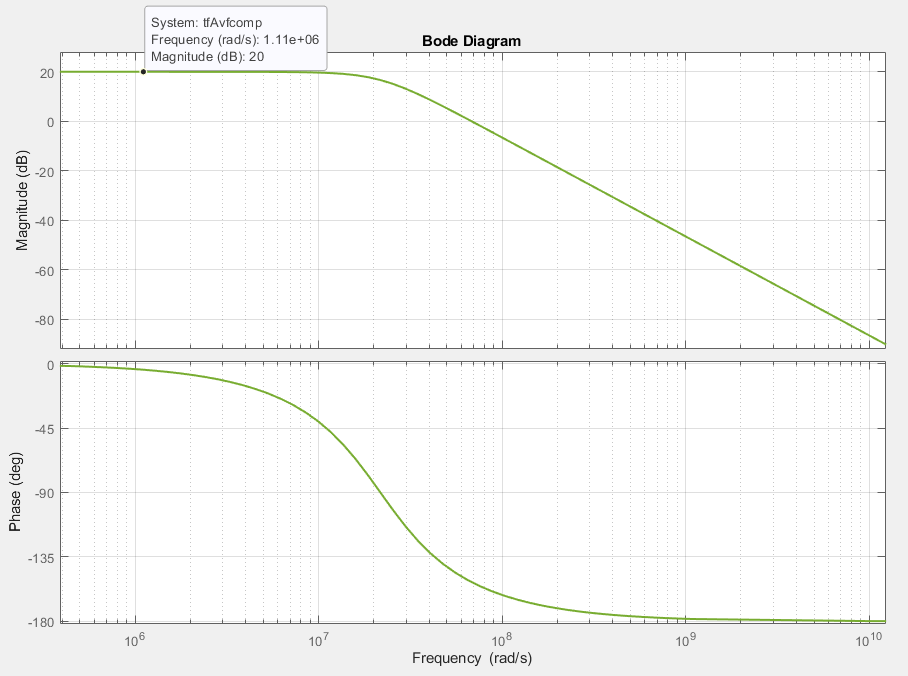
\includegraphics[width=0.9\linewidth]{figuras/9. comp_feedback.png}
    \caption{Diagrama de Bode del amplificador compuesto realimentado}
\end{figure}

\begin{figure}[H]
    \centering
    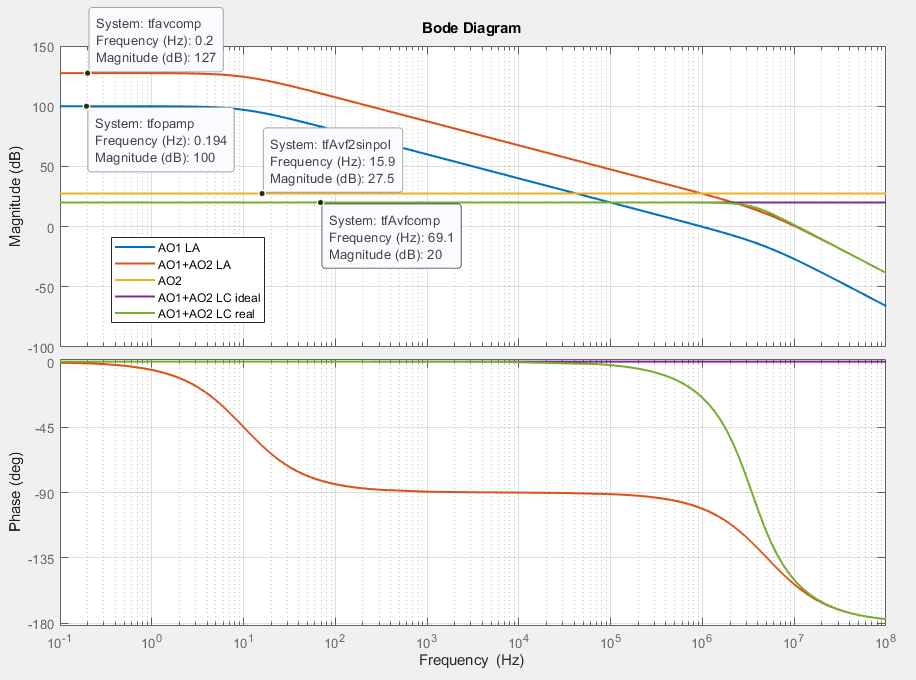
\includegraphics[width=0.9\linewidth]{figuras/10. BODE.png}
    \caption{Diagrama de Bode del amplificador VFA-VFA}
    \label{fig:foto}
        \begin{description} [itemsep=1pt, parsep=0pt, partopsep=0pt, topsep=0pt]
         \centering
         \small
         \item[Azul:]  Ganancia de AO1 a lazo abierto.
         \item[Amarillo:]  Ganancia de AO2 a lazo abierto.
         \item[Naranja:]  Ganancia del amplificador compuesto a lazo abierto.
         \item[Violeta:]  Ganancia del amplificador compuesto a lazo cerrado ideal.
         \item[Verde:]  Ganancia del amplificador compuesto a lazo cerrado real.
        \end{description}
\end{figure}


\hspace{1mm} A través del código de Matlab, se pudo comprobar que la ganancia de lazo cerrado es igual a $Avf_2=27.5~dB$ y la ganancia del amplificador compuesto a lazo abierto resulta ser $127.5~dB$. Con estos valores, se puede calcular el valor del polo $f_g$.


\begin{equation}
    \frac{127.21~dB-20~dB}{log(10)-log(f_g)}=-20~dB/dec
\end{equation}

 
\hspace{1mm} Despejando $f_g$, se obtiene:

\begin{equation}
    f_g=2.29~MHz
\end{equation}




\subsection{Simulación}
\hspace{1mm} Luego de todos los cálculos realizados, se procedió a simular el circuito para comparar y verificar los resultados. Para ello, se utilizó LTspice XVII. El circuito fue el siguiente:

\begin{figure}[H]
    \centering
    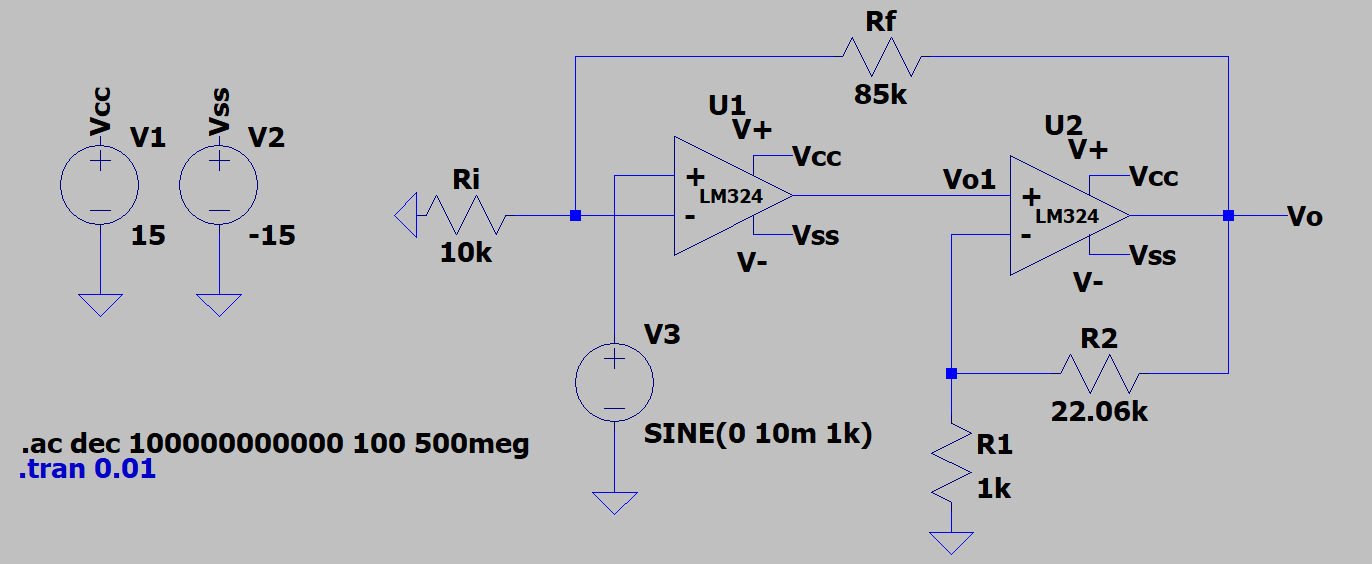
\includegraphics[width=0.9\linewidth]{figuras/Circuito1.png}
    \caption{Circuito VFA - VFA}
\end{figure}

\hspace{1mm} Primero, se evaluó la ganancia del sistema, para lo cual fue necesario graficar tanto la señal de entrada como la de salida. Con una entrada de $10~mV$, se obtuvo una salida de $92.87~mV$, lo que resulta en una ganancia de:
\begin{equation*}
    G = \frac{V_{out}}{V_{in}}=\frac{92.87~mV}{10~mv}
\end{equation*}
\begin{equation*}
    \boxed{G = 9.287}
\end{equation*}

\hspace{1mm} Esto implica un error del $7.13\%$ aproximadamente. 

\begin{figure}[H]
    \centering
    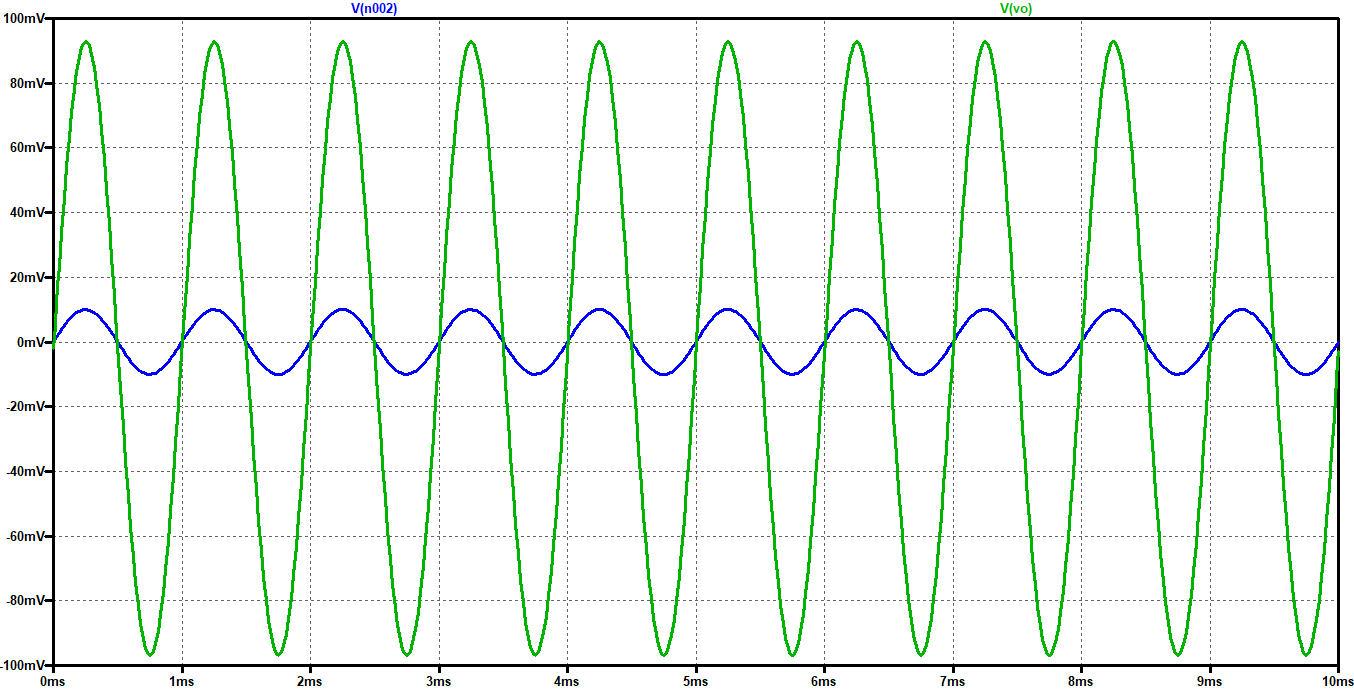
\includegraphics[width=0.9\linewidth]{figuras/Ganancia_c1.png}
    \caption{Ganancia del circuito VFA - VFA}
\end{figure}
 
\hspace{1mm} Posteriormente, se simuló la respuesta en frecuencia. Se obtuvo una ganancia de $20~dB$ y una frecuencia de corte en $134.44 KHz$, la cual se presenta en una caída de $-3~dB$. Esto representa un error del $34\%$ en comparación con lo simulado en Matlab.

\begin{figure} [H]
    \centering
    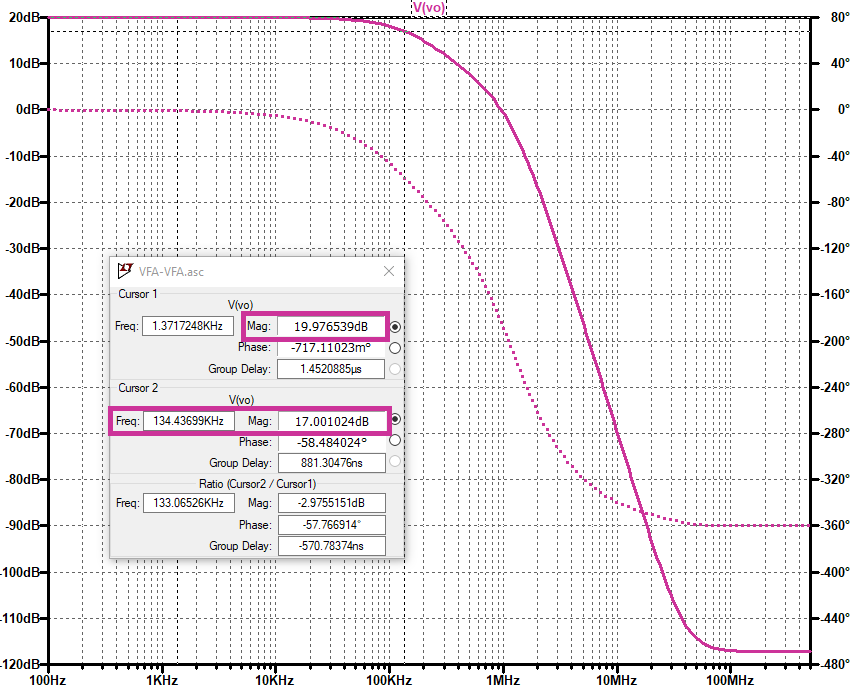
\includegraphics[width=0.9\linewidth]{figuras/Bode_c1.png}
    \caption{Diagrama de Bode del circuito VFA - VFA}
\end{figure}



\subsection{Conclusiones}
\hspace{1mm} En este apartado, se analizaron las ganancias de lazo abierto, lazo cerrado y total de un amplificador VFA-VFA, combinando cálculos teóricos y simulaciones tanto en Matlab como en LTspice XVII. Los resultados teóricos establecieron los valores de resistencias necesarios para alcanzar una ganancia de \(20~dB\) a lazo cerrado.

\bigskip
\hspace{1mm} Las simulaciones en LTspice XVII confirmaron el diseño, aunque con algunos errores en comparación con los resultados teóricos: un $7.13\%$ en la ganancia y un $34\%$ en la respuesta en frecuencia. Sin embargo, tanto el análisis teórico como las simulaciones proporcionan una base sólida para la implementación del amplificador. Estas diferencias destacan la importancia de combinar el análisis teórico con simulaciones en diversas herramientas, lo que permite ajustar y validar el diseño del circuito para garantizar su rendimiento en condiciones reales.
